%% BioMed_Central_Tex_Template_v1.06
%%                                      %
%  bmc_article.tex            ver: 1.06 %
%                                       %

%%IMPORTANT: do not delete the first line of this template
%%It must be present to enable the BMC Submission system to
%%recognise this template!!

%%%%%%%%%%%%%%%%%%%%%%%%%%%%%%%%%%%%%%%%%
%%                                     %%
%%  LaTeX template for BioMed Central  %%
%%     journal article submissions     %%
%%                                     %%
%%          <8 June 2012>              %%
%%                                     %%
%%                                     %%
%%%%%%%%%%%%%%%%%%%%%%%%%%%%%%%%%%%%%%%%%


%%%%%%%%%%%%%%%%%%%%%%%%%%%%%%%%%%%%%%%%%%%%%%%%%%%%%%%%%%%%%%%%%%%%%
%%                                                                 %%
%% For instructions on how to fill out this Tex template           %%
%% document please refer to Readme.html and the instructions for   %%
%% authors page on the biomed central website                      %%
%% http://www.biomedcentral.com/info/authors/                      %%
%%                                                                 %%
%% Please do not use \input{...} to include other tex files.       %%
%% Submit your LaTeX manuscript as one .tex document.              %%
%%                                                                 %%
%% All additional figures and files should be attached             %%
%% separately and not embedded in the \TeX\ document itself.       %%
%%                                                                 %%
%% BioMed Central currently use the MikTex distribution of         %%
%% TeX for Windows) of TeX and LaTeX.  This is available from      %%
%% http://www.miktex.org                                           %%
%%                                                                 %%
%%%%%%%%%%%%%%%%%%%%%%%%%%%%%%%%%%%%%%%%%%%%%%%%%%%%%%%%%%%%%%%%%%%%%

%%% additional documentclass options:
%  [doublespacing]
%  [linenumbers]   - put the line numbers on margins

%%% loading packages, author definitions

%\documentclass[twocolumn]{bmcart}% uncomment this for twocolumn layout and comment line below
\documentclass{bmcart}

\setlength{\marginparwidth}{3.5cm} % to give space for margin notes - remove on submission

%%% Load packages
\usepackage{amsthm,amsmath}
%\RequirePackage{natbib}
%\RequirePackage[authoryear]{natbib}% uncomment this for author-year bibliography
%\RequirePackage{hyperref}
\usepackage[utf8]{inputenc} %unicode support
%\usepackage[applemac]{inputenc} %applemac support if unicode package fails
%\usepackage[latin1]{inputenc} %UNIX support if unicode package fails
\usepackage{todonotes}
\usepackage{tabularx}
\usepackage{booktabs}
\usepackage{multirow}

%%%%%%%%%%%%%%%%%%%%%%%%%%%%%%%%%%%%%%%%%%%%%%%%%
%%                                             %%
%%  If you wish to display your graphics for   %%
%%  your own use using includegraphic or       %%
%%  includegraphics, then comment out the      %%
%%  following two lines of code.               %%
%%  NB: These line *must* be included when     %%
%%  submitting to BMC.                         %%
%%  All figure files must be submitted as      %%
%%  separate graphics through the BMC          %%
%%  submission process, not included in the    %%
%%  submitted article.                         %%
%%                                             %%
%%%%%%%%%%%%%%%%%%%%%%%%%%%%%%%%%%%%%%%%%%%%%%%%%


%\def\includegraphic{}
%\def\includegraphics{}



%%% Put your definitions there:
\startlocaldefs
\newcommand{\PR}{{\mathsf P}}
\endlocaldefs


%%% Begin ...
\begin{document}

%%% Start of article front matter
\begin{frontmatter}

\begin{fmbox}
\dochead{Research}

%%%%%%%%%%%%%%%%%%%%%%%%%%%%%%%%%%%%%%%%%%%%%%
%%                                          %%
%% Enter the title of your article here     %%
%%                                          %%
%%%%%%%%%%%%%%%%%%%%%%%%%%%%%%%%%%%%%%%%%%%%%%

\title{Three-outcome designs for external pilot trials with progression criteria}

%%%%%%%%%%%%%%%%%%%%%%%%%%%%%%%%%%%%%%%%%%%%%%
%%                                          %%
%% Enter the authors here                   %%
%%                                          %%
%% Specify information, if available,       %%
%% in the form:                             %%
%%   <key>={<id1>,<id2>}                    %%
%%   <key>=                                 %%
%% Comment or delete the keys which are     %%
%% not used. Repeat \author command as much %%
%% as required.                             %%
%%                                          %%
%%%%%%%%%%%%%%%%%%%%%%%%%%%%%%%%%%%%%%%%%%%%%%

\author[
   addressref={aff1},                   % id's of addresses, e.g. {aff1,aff2}
   email={d.t.wilson@leeds.ac.uk}   % email address
]{\inits{DTW}\fnm{Duncan T} \snm{Wilson}}
\author[
   addressref={aff1},
   email={john.RS.Smith@cambridge.co.uk}
]{\inits{JRS}\fnm{John RS} \snm{Smith}}

%%%%%%%%%%%%%%%%%%%%%%%%%%%%%%%%%%%%%%%%%%%%%%
%%                                          %%
%% Enter the authors' addresses here        %%
%%                                          %%
%% Repeat \address commands as much as      %%
%% required.                                %%
%%                                          %%
%%%%%%%%%%%%%%%%%%%%%%%%%%%%%%%%%%%%%%%%%%%%%%

\address[id=aff1]{%                           % unique id
  \orgname{Clinical Trials Research Unit, Leeds Institute of Clinical Trials Research, University of Leeds}, % university, etc
  %\street{Waterloo Road},                     %
  \postcode{LS2 9JT}                                % post or zip code
  \city{Leeds},                              % city
  \cny{UK}                                    % country
}

%%%%%%%%%%%%%%%%%%%%%%%%%%%%%%%%%%%%%%%%%%%%%%
%%                                          %%
%% Enter short notes here                   %%
%%                                          %%
%% Short notes will be after addresses      %%
%% on first page.                           %%
%%                                          %%
%%%%%%%%%%%%%%%%%%%%%%%%%%%%%%%%%%%%%%%%%%%%%%

%\begin{artnotes}
%\note{Sample of title note}     % note to the article
%\note[id=n1]{Equal contributor} % note, connected to author
%\end{artnotes}

\end{fmbox}% comment this for two column layout

%%%%%%%%%%%%%%%%%%%%%%%%%%%%%%%%%%%%%%%%%%%%%%
%%                                          %%
%% The Abstract begins here                 %%
%%                                          %%
%% Please refer to the Instructions for     %%
%% authors on http://www.biomedcentral.com  %%
%% and include the section headings         %%
%% accordingly for your article type.       %%
%%                                          %%
%%%%%%%%%%%%%%%%%%%%%%%%%%%%%%%%%%%%%%%%%%%%%%

\begin{abstractbox}

\begin{abstract} % abstract
The decision of if and how to progress to a definitive trial following a pilot study is often guided by quantitative progression criteria with three possible outcomes, but there is little methodological work examining how they, or the pilot sample size, should be determined. We review three-outcome designs originally proposed for phase II trials and consider if they can provide a formal statistical framework for pilot trials. We conclude that, from a statistical perspective, there are limited benefits from using quantitative three-outcome progression criteria in pilot trials.

\parttitle{Background} %if any
the context and purpose of the study.

\parttitle{Methods} %if any
how the study was performed and statistical tests used.

\parttitle{Results} %if any
the main findings.

\parttitle{Conclusions} %if any
brief summary and potential implications.
\end{abstract}

%%%%%%%%%%%%%%%%%%%%%%%%%%%%%%%%%%%%%%%%%%%%%%
%%                                          %%
%% The keywords begin here                  %%
%%                                          %%
%% Put each keyword in separate \kwd{}.     %%
%%                                          %%
%%%%%%%%%%%%%%%%%%%%%%%%%%%%%%%%%%%%%%%%%%%%%%

\begin{keyword}
\kwd{pilot}
\kwd{progression criteria}
\kwd{sample size}
\end{keyword}

% MSC classifications codes, if any
%\begin{keyword}[class=AMS]
%\kwd[Primary ]{}
%\kwd{}
%\kwd[; secondary ]{}
%\end{keyword}

\end{abstractbox}
%
%\end{fmbox}% uncomment this for twcolumn layout

\end{frontmatter}

%%%%%%%%%%%%%%%%%%%%%%%%%%%%%%%%%%%%%%%%%%%%%%
%%                                          %%
%% The Main Body begins here                %%
%%                                          %%
%% Please refer to the instructions for     %%
%% authors on:                              %%
%% http://www.biomedcentral.com/info/authors%%
%% and include the section headings         %%
%% accordingly for your article type.       %%
%%                                          %%
%% See the Results and Discussion section   %%
%% for details on how to create sub-sections%%
%%                                          %%
%% use \cite{...} to cite references        %%
%%  \cite{koon} and                         %%
%%  \cite{oreg,khar,zvai,xjon,schn,pond}    %%
%%  \nocite{smith,marg,hunn,advi,koha,mouse}%%
%%                                          %%
%%%%%%%%%%%%%%%%%%%%%%%%%%%%%%%%%%%%%%%%%%%%%%

%%%%%%%%%%%%%%%%%%%%%%%%% start of article main body
% <put your article body there>

%%%%%%%%%%%%%%%%
%% Background %%
%%
\section{Introduction}\label{sec:introduction}

When there is some uncertainty about the feasibility of a planned randomised clinical trial (RCT), an external pilot trial can be conducted in advance. External pilots take the form of a smaller version of the main trial \cite{Eldridge2016}, and can be used to estimate various parameters of interest when deciding if (and how) to progress to the main study. Investing in a pilot trial can identify potential issues at an early stage, making a successful main trial more likely and reducing overall research waste \cite{Morgan2018}.

Progression decisions are often guided by so-called \emph{progression criteria} \cite{Eldridge2016a}. A single two-outcome progression criterion specifies a decision rule which maps the pilot data to a \emph{stop} or \emph{go} outcome. Specifically, the pilot data are used to calculate a statistic, typically an estimate of a parameter of interest, and this statistic is compared against a threshold value. If the statistic exceeds the threshold, the suggested decision is to \emph{go} forward to the main trial; otherwise, to \emph{stop} on the grounds of infeasibility. When progression criteria are specified for several parameters, these can be combined by proceeding to the main trial only if all of the estimates exceed their respective thresholds. It has been recommended that, in addition to being reported in the pilot study manuscript, progression criteria are pre-specified at the protocol stage in agreement with the study funder \cite{NIHR2017, Mbuagbaw2019}.

It has become common for progression criteria to be based on a three-outcome `traffic light' system \cite{Avery2017}. These criteria stipulate two threshold values for a given parameter of interest. If the estimate falls below the lower of these, the decision is to stop (red); if the estimate falls above the higher threshold, the decision is to proceed immediately to the main trial (green); and if the estimate falls between the two thresholds, an intermediate decision is reached (amber). The specific purpose and interpretation of this intermediate decision can vary, and will depend on the motivation for using the three-outcome system. Three such motivations can be found in the methodological literature. Firstly, it has been argued that making strict stop/go decisions based on a single threshold  may lead to an unacceptably high chance of making the wrong decision as a result of sampling variability \footnote{``\emph{\ldots estimates of rates in pilot trials may be subject to considerable uncertainty, so that it is best to be cautious about setting definitive thresholds that could be missed simply due to chance variation. In fact it is becoming increasingly common for investigators to use a traffic light system for criteria used to judge feasibility\ldots}''} \cite{Eldridge2016a}. By allowing for an intermediate result in between \emph{stop} and \emph{go}, the probability of incorrect decisions may be reduced.

%This argument is paralled in the three outcome literaure, which argue that the designs can improve efficiency and either increase power, or reduce the required sample size.

A second motivation stems from the fact that many aspects (quantitative and qualitative) being studied in a pilot trial are potentially relevant to the progression decision, and that this decision will be jointly made by several stakeholders (such as the trial team, the trial steering commitee, and the funder)\todo{Noting that it's not just opening up to other information, but also facilitating a joint decision making process}. A three-outcome system will allow immediate \emph{stop} or \emph{go} decisions to be made if the evidence is sufficiently strong with respect to a handful of key parameters, whilst allowing, in the event of a borderline result, the decision to be informed by other data based on the differing perspectives of all decision makers. It has been argued that this system better represents what happens in practice even when a two-outcome process is nominally being followed. In that case, although a borderline result will technically dictate a firm \emph{stop/go} decision, this may be overridden in light of other information \cite{Sargent2001}.\todo{Coming back to this in the discussion - question of whether three outcome designs should be routinely used over two-outcome, since they better reflect actual practice.}

A final reason for an intermediate outcome is to provide the flexibility needed to make some adjustment to the intervention or trial design in an attempt to improve the parameter in question and ensure the feasibility of the main trial\footnote{``\emph{In amber situations, there may be remediable issues that would otherwise prevent progression to the main trial but that, if identified early enough, can be addressed to the satisfaction of those reviewing progress in order for the trial to continue to a main trial.}''} \cite{Avery2017}. For example, after observing a mediocre follow-up rate in a pilot trial, we might consider moving from a postal follow-up strategy to one based on contacting the participants over the phone. A three-outcome approach could facilitate this by prescribing an `adjustment' decision to the intermediate outcome, whilst still allowing for immediate stopping or progression when obtaining `stop' or `go' outcomes. This approach is somewhat in line with guidance on the development and evaluation of complex interventions \cite{Craig2008}\todo{Need to update to latest guidance} which emphasises the iterative nature of the process and the likely need to adjust the original intervention or trial design before conducting the main trial.

Despite the prevalence of quantitative three-outcome progression criteria\cite{Herbert2019}, there is little statistical guidance to help researchers decide how they should be specified. The related question of determining the pilot trial sample size is also undeveloped, with work in this area typically focusing on pilot trials where the primary objective is to estimate the primary outcome variance to inform the main trial sample size calculation. These methods are nevertheless used when this is not the main purpose of the pilot, often in the form of simple `rules-of-thumb' \cite{Browne1995, Teare2014, Whitehead2015}. Three-outcome designs have, however, been proposed for phase II trials of cancer treatments \cite{Kirby2016}. Some of these designs were motivated by the same factors given above, and so may provide a useful framework for the design and analysis of pilot trials with three-outcome progression criteria.

In this paper we consider if, and how, three-outcome phase II designs can be used to determine optimal progression criteria and sample size in pilot trials. We begin by introducing a simple example in Section \ref{sec:example}. In Section \ref{sec:tests} we argue that quantitative progression criteria are mathematically equivalent to hypothesis tests, and are best viewed as such. We then review relevant three-outcome phase II trial designs and extend these to the pilot trial setting in Section \ref{sec:review}. In Section \ref{sec:methods} we examine the statistical properties of these pilot trial designs and consider whether or not they can help achieve any of the three motivating goals. Finally, we conclude with a discussion in Section \ref{sec:discussion}.

\section{An example}\label{sec:example}

Throughout this article we will refer to a simple example of a pilot trial assessing the probability that a participant in the intervention arm of the main trial will adhere to their prescribed treatment. Specifically, we consider adherence to be measured as a binary outcome and denote the probability of adherence by $\rho$. Given  $n$ patients in the pilot trial's intervention arm, we then model the number of adherers using a binomial distribution with parameters $\rho$ and $n$. We denote the pilot estimate by $\hat{\rho}$.

We will consider both two- and three-outcome versions of progression criteria. In the two-outcome case, the progression decision is defined by a threshold value $x$, such that
\begin{equation}\label{eqn:two_outcome}
\text{Decision} = 
\begin{cases}
\text{\emph{go}} & \text{ if } \hat{\rho} \geq x \\
\text{\emph{stop}} & \text{ if } \hat{\rho} < x. \\
\end{cases}
\end{equation}

In the three-outcome case, we allow for an additional intermediate result and require two thresholds, $x_0$ and $x_1$:
\begin{equation}\label{eqn:three_outcome}
\text{Decision} = 
\begin{cases}
\text{\emph{go}} & \text{ if } \hat{\rho} \geq x_1 \\
\text{\emph{pause}} & \text{ if } x_0 < \hat{\rho} < x_1 \\
\text{\emph{stop}} & \text{ if } \hat{\rho} < x_0. \\
\end{cases}
\end{equation}
The specific meaning of the intermediate \emph{pause} result will vary depending on the purpose and context of the pilot trial. 

\section{Progression criteria as hypothesis tests}\label{sec:tests}

In order to apply the two-outcome progression criteria of Equation \ref{eqn:two_outcome}, we must choose the sample size $n$ and the threshold $x$. One way to do so is though constructing a hypothesis test using the approach of A'Hern \cite{AHern2001}, as follows. First, we identify a parameter value $\rho_0$ such that if $\rho \leq \rho_0$ we would like to limit the probability of incorrectly making a `go' decision (a type I error) to at most $\alpha^*$. Similarly, we identify $\rho_1$ such that if $\rho \geq \rho_1$ we would like to limit the probability of incorrectly making a `stop' decision (a type II error) to at most $\beta^*$. For example, we could choose adherence rates of $\rho_0 = 0.5$ and $\rho_1 = 0.7$ to represent poor and promising values respectively, and then use the standard choices of $\alpha^* = 0.05, \beta^* = 0.1$ for our nominal error rates. We then choose values of $n$ and $x$ which minimise $n$ whilst satisfying the type I and II error rate constraints
\begin{align}
\alpha &= \max_{\rho \leq \rho_0} \PR[ \hat{\rho} > x ~ | ~ \rho] \\
&= \PR[ \hat{\rho} > x ~ | ~ \rho = \rho_0] \leq \alpha^* \\
\beta &= \max_{\rho \geq \rho_1} \PR[ \hat{\rho} \leq x ~ | ~ \rho] \\
&= \PR[ \hat{\rho} \leq x ~ | ~ \rho = \rho_1] \leq \beta^*,
\end{align}
where we have used the monotonicity of power as a function of $\rho$ to note that the type I and II error rates will be maximised when $\rho = \rho_0$ and $\rho = \rho_1$ respectively.\todo{We have defined a one-sided type I error here without drawing attention to it - seems OK to me as it's a natural view when thinking about progression decisions. I think wait and see if a reviewer wants this to be justified / discussed.}

Alternatively, we can work backwards and take any given choice for $n$ and $x$ and calculate the resulting error rates for some hypotheses $\rho_0, \rho_1$. In particular, whenever a pilot trial progression criteria is specified in the form of Equation \ref{eqn:two_outcome}, it is mathematically equivalent to a hypothesis test. For example, consider a pilot trial with $n = 15$ participants in the intervention arm and a \emph{stop/go} progression criteria with threshold $x = 9/15$. If we suppose that the null and alternative hypotheses are $\rho_0 = 0.5, \rho_1 = 0.7$, this design will give type I and II error rates of $\alpha = 0.28$ and $1 - \beta = 0.72$. If we instead constrain the error rates to, for example, $\alpha^* = 0.05$ and $\beta^* = 0.1$, the smallest possible sample size is $n = 53$ and the corresponding progression threshold is $x = 32/48$. 

The equivalence of two-outcome progression criteria and hypothesis tests suggests the latter can provide a statistical framework for determining the former \cite{Lewis2021a}. This will allow us to express what parameter values would lead to errors of each type\todo{Return in discussion to the difficulty in doing this compared with determining an efficacy null hypothesis}, and then subsequently to control the probability of these errors by choosing a sufficient sample size.

\section{Extending three-outcome phase II trial designs}\label{sec:review}

Just as standard hypothesis testing can be used as a framework for two-outcome progression criteria, three-outcome extensions of it can be used for the three-outcome progression criteria of Equation \ref{eqn:three_outcome}. We will consider two such extensions proposed for phase II trials by Sargent \emph{et al.} \cite{Sargent2001} and by Storer \cite{Storer1992}.

The design of Sargent \emph{et al.} defines four operating characteristics relevant to the three-outcome setting. Firstly, a measure akin to the type I error rate, denoted $\alpha_a$, is defined as the probability under the null hypothesis $\rho = \rho_0$ that the parameter estimate will exceed the upper threshold $x_1$ and thereby lead to a \emph{go} decision. Similarly, a type II error rate $\beta_a$ is given as the probability, under the alternative hypothesis $\rho = \rho_1$, of the parameter estimate failing below the lower threshold $x_0$ and leading to a \emph{stop} decision. Two further operating characteristics relating to the intermediate outcome are then defined: the probability of obtaining a \emph{pause} decision under then null hypothesis, denoted $\lambda$, and again under the alternative hypothesis, denoted $\gamma$. These operating characteristics are summarised in Table \ref{tab:ocs} and illustrated in Figure \ref{fig:Sarg_ocs}. The authors propose to set constraints on these four operating characteristics and choose $n, x_0,$ and $x_1$ to minimise $n$ whilst satisfying these constraints. They argue that their designs will lead to a lower sample size requirement than standard two-outcome alternatives.

\begin{table}
\caption{Operating characteristics for Sargent \emph{et al.} and Storer's three-outcome designs \cite{Sargent2001, Storer1992}.}
\begin{tabularx}{\textwidth}{l l l X}
\toprule
 & Symbol & Equation & Description \\
\midrule
\multirow{6}{*}{\rotatebox[origin=c]{90}{Sargent}} & $\alpha_a$ & $\PR[ \hat{\rho} > x_1 | \rho = \rho_0]$ & Probability of an immediate \emph{go} decision under the null hypothesis \\
 & $\beta_a$ & $\PR[ \hat{\rho} \leq x_0 | \rho = \rho_1]$ & Probability of an immediate \emph{stop} decision under the alternative hypothesis \\
 & $\lambda$ & $\PR[ x_0 < \hat{\rho} \leq x_1 | \rho = \rho_0]$ & Probability of a \emph{pause} decision under the null hypothesis \\
 & $\delta$ & $\PR[ x_0 < \hat{\rho} \leq x_1 | \rho = \rho_1]$ &  Probability of a \emph{pause} decision under the alternative hypothesis \\
 &&& \\
\multirow{6}{*}{\rotatebox[origin=c]{90}{Storer}} & $\alpha_b$ & $\PR[ \hat{\rho} > x_0 | \rho = \rho_0]$ & Probability of not obtaining an immediate \emph{stop} decision under the null hypothesis \\
 & $\beta_b$ & $\PR[ \hat{\rho} \leq x_1 | \rho = \rho_1]$ & Probability of not obtaining an immediate \emph{go} decision under the alternative hypothesis \\
 & $\gamma_L$ & $\PR[ \hat{\rho} \leq x_0 | \rho = \rho']$ & Probability of an immediate \emph{stop} decision when $\rho = \rho'$ \\
 & $\gamma_U$ & $\PR[ x_1 < \hat{\rho} | \rho = \rho']$ &  Probability of an immediate \emph{go} decision when $\rho = \rho'$ \\
\bottomrule
\end{tabularx}
\label{tab:ocs}
\end{table}

\begin{figure}
\centering
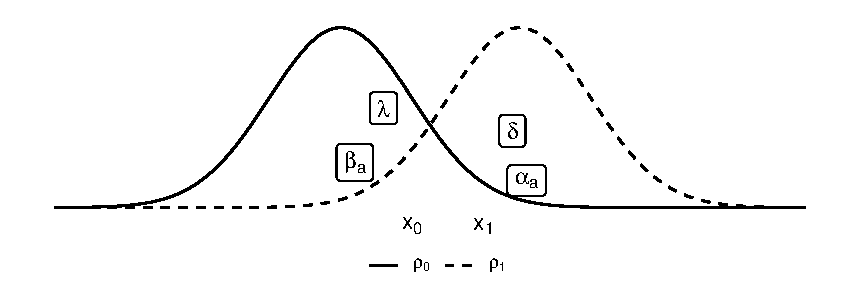
\includegraphics[scale=0.8]{./figures/Sarg_ocs}
\caption{Graphical illustration of the operating characteristics for Sargent \emph{et al.}'s three-outcome design \cite{Sargent2001}. The curves represents the sampling distribution of the estimate under the null hypothesis $\rho = \rho_0$ (solid line) and the alternative hypothesis $\rho = \rho_1$ (dashed line).}
\label{fig:Sarg_ocs}
\end{figure}

An alternative three-outcome design proposed by Storer \cite{Storer1992} takes the same basic approach, but with a different set of four operating characteristics. Here, the type I error rate $\alpha_b$ is taken to be the probability of exceeding the lower threshold, $x_0$, under the null; and similarly the type II error rate $\beta_b$ is now the probability of failing to exceed the upper threshold under the alternative. The remaining two operating characteristics are the probabilities of incorrectly obtaining a \emph{stop} or a \emph{go} decision when the true parameter is at some midpoint $\rho' \in (\rho_0, \rho_1)$. These operating characteristics, denoted by $\gamma_L$ and $\gamma_U$ respectively, reflects the motivation of this design to \emph{encourage} an intermediate outcome when the true parameter value is between the null and alternative. The operating characteristics are summarised in Table \ref{tab:ocs} and illustrated in Figure \ref{fig:Stor_ocs}, where we follow the author's suggestion to set $\rho' = (\rho_1 + \rho_0)/2$.

\begin{figure}
\centering
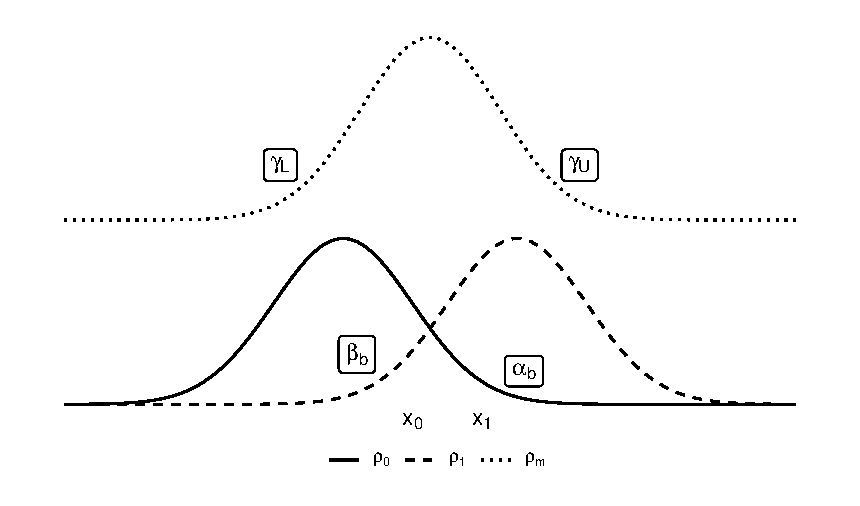
\includegraphics[scale=0.8]{./figures/Stor_ocs}
\caption{Graphical illustration of the operating characteristics for Storer's three-outcome design\cite{Storer1992}. The curves represents the sampling distribution of the estimate under the null hypothesis $\rho = \rho_0$ (solid line), the alternative hypothesis $\rho = \rho_1$ (dashed line), and a mid point $\rho = (\rho_1 + \rho_0)/2$ (dotted line).}
\label{fig:Stor_ocs}
\end{figure}

Considering the proposal of Sargent \emph{et al.}, we note that the measure $\alpha_a$ does not fully capture the probability of making a type I error \footnote{Sargent \emph{et al.}  state that ``We  can interpret $\alpha$ in the usual  manner,  i.e., the  maximum probability of making an erroneous decision by rejecting the null hypothesis when in fact it is true'', although then go on to say ``However, the error rates $\alpha$ and $\beta$ in a three-outcome design cannot be viewed in the same way as in the traditional two-outcome design."} since a decision to progress to the main trial can be arrived at in two ways: directly, by obtaining $\hat{\rho} > x_1$; or indirectly, by first obtaining a \emph{pause} outcome $x_0 < \hat{\rho} < x_1$ and then deciding to proceed. To capture these situations, we first define the probabilities of making incorrect decisions following a \emph{pause} outcome under the null and alternative hypotheses:
\begin{align}
\eta_0 &= \PR[\text{decide to \emph{go}} ~|~ \rho = \rho_0, x_0 < \hat{\rho} \leq x_1] \\
\eta_1 &= \PR[\text{decide to \emph{stop}} ~|~ \rho = \rho_1, x_0 < \hat{\rho} \leq x_1].
\end{align}
For example, $\eta_0$ is the probability of making a \emph{go} decision following a \emph{pause} outcome and when the true parameter value is $\rho_0$. The probability of making a \emph{go} decision when $\rho = \rho_0$, then, is not $\alpha_a$ but
$$
\alpha = \alpha_a + \eta_0 \lambda.
$$
Similarly, the type II error rate is
$$
\beta = \beta_a + \eta_1 \delta.
$$
These operating characteristics have been suggested previously in the context of multi-armed screening trials \cite{Sargent2001a, Dehbi2020}. For simplicity we will assume that $\eta_0 = \eta_1 = \eta$; that is, the probability of eventually making the wrong decision following an intermediate result is the same when $\rho = \rho_0$ as when $\rho = \rho_1$. Under this reformulation an optimal three-outcome design can be found by first estimating the probability $\eta$, setting constraints on the type I and II error rates $\alpha, \beta$, and finally searching for the values of  $n, x_0, x_1$ which minimise $n$ whilst satisfying the constraints. Note that we no longer need to set constraints on the operating characteristics $\delta$ and $\lambda$, as the probability of obtaining an intermediate decision under the null and alternative hypothesis will be automatically limited by the constraints on $\alpha$ and $\beta$ respectively.\todo{Is this clear or does it need more explanation / discussion?}

A similar argument applies when considering Storer's method, where we can replace the operating characteristics $\alpha_b, \beta_b$ with $\alpha$ and $\beta$. As the operating characteristics $\gamma_L, \gamma_U$ are designed to encourage an intermediate outcome under $\rho_m$, rather than limit it as in the method of Sargent \emph{et al.}, we keep these in our reformulation. Thus, an optimal three-outcome design under the reformulated Storer method can be found by estimating the probability $\eta$, setting constraints on $\alpha, \beta, \gamma_L$ and $\gamma_U$, and finally searching for the values of  $n, x_0, x_1$ which minimise $n$ whilst satisfying the constraints. 

For simplicity, we will assume that the cost of an incorrect \emph{stop} or \emph{go} decision when $\rho = \rho'$ are the same, and replace the two error rates $\gamma_U, \gamma_L$ by the single error rate
$$
\gamma = \gamma_L + \gamma_U,
$$
the probability of making an incorrect conclusive decision of either type. Note that the reformulated method of Sargent \emph{et al.} is a special case of this method when we set the trivial constraint $\gamma \leq 1$, and so we have a single unified framework for designing and analysing three-outcome studies.

\subsection{Allowing adjustments}\label{sec:adjustments}

We now further generalise the three-outcome testing framework to allow for adjustments to be made following a \emph{pause} outcome. Denote the main trial parameter by $\rho_m$, so that $\rho_m = \rho$ if no adjustment is made and $\rho_m  = \rho + \tau$ if it is. We will assume that the adjustment effect $\tau$ is known up to an interval $\tau \in [\tau_{min}, \tau_{max}]$, and that $\tau_{min} \geq 0$. We then refine our definitions of the error rates $\alpha$ and $\beta$ as

\begin{itemize}
\item $\alpha$: the probability of proceeding to the main trial when $\rho_m \leq \rho_0$
\item $\beta$: the probability of not proceeding to the main trial when $\rho_m \geq \rho_1$;
\end{itemize}

Because we can make a \emph{go} decision in two ways, $\alpha$ is now the maximum probability of proceeding either directly or following an \emph{pause} outcome (in which case the adjustment is made) when this will lead to $\rho_m \leq \rho_0$. As before, we assume there is a constant probability of mistakenly deciding to proceed following a \emph{pause} outcome when in fact $\rho + \tau \leq \rho_0$, denoted  by $\eta$. That is,

$$
\alpha = \max \left[ \max_{\rho \leq \rho_0} \PR(x_1 < \hat{\rho}), \max_{\rho + \tau \leq \rho_0} \eta \PR(x_0 < \hat{\rho} \leq x_1) + \PR(x_1 < \hat{\rho}) \right].
$$

The first term is maximised at $\rho = \rho_0$. The second term can be written as
$$
\begin{aligned}
\eta \PR(x_0 < \hat{\rho} \leq x_1) + \PR(x_1 < \hat{\rho}) &=
\eta \PR(\hat{\rho} \leq x_1) - \eta \PR(\hat{\rho} \leq x_0) + 1 - \PR(\hat{\rho} \leq x_1)\\
&= 1 + (\eta - 1)\PR(\hat{\rho} \leq x_1) - \eta \PR(\hat{\rho} \leq x_0),
\end{aligned}
$$
and so is maximised at $\rho = \rho_0 - \tau_{min}$, giving 

\begin{equation}\label{eqn:alpha}
\alpha = \max \left[ \PR(x_1 < \hat{\rho} ~|~ \rho = \rho_0), \eta \PR(x_0 < \hat{\rho} \leq x_1 ~|~ \rho = \rho_0 - \tau_{min}) + \PR(x_1 < \hat{\rho} ~|~ \rho = \rho_0 - \tau_{min}) \right].
\end{equation}

An incorrect \emph{stop} decision may again occur two ways - directly, or following a \emph{pause} outcome. The error rate $\beta$ can therefore be written as

\begin{equation}\label{eqn:beta_a}
\beta = \max \left[ \max_{\rho > \rho_1} \PR(\hat{\rho} \leq x_0), \max_{\rho + \tau > \rho_1} \PR(\hat{\rho} \leq x_0) + \eta \PR(x_0 < \hat{\rho} \leq x_1) \right],
\end{equation}

where we have assumed the same probability of an incorrect decision following a \emph{pause} outcome as with the $\alpha$ case. The first term is maximised at $\rho = \rho_1$, while the second term can be written as
$$
\eta \PR(\hat{\rho} \leq x_1) + (1 - \eta) \PR(\hat{\rho} \leq x_0),
$$
which is maximised at $\rho = \rho_1 - \tau_{max}$. Since $\tau_{max} > 0$, then $\PR(\hat{\rho} \leq x_0 | \rho = \rho_1) \leq \PR(\hat{\rho} \leq x_0 ~|~ \rho = \rho_1  - \tau_{max})$ and so Equation \ref{eqn:beta_a} can be simplified to

\begin{equation}\label{eqn:beta}
\beta = \PR(\hat{\rho} \leq x_0 ~|~ \rho = \rho_1 - \tau_{max}) + \eta \PR(x_0 < \hat{\rho} \leq x_1 ~|~ \rho = \rho_1 - \tau_{max}).
\end{equation}

Note that the general error rates of Equations \ref{eqn:alpha} and \ref{eqn:beta} are valid in the special case where no adjustments are going to be made following a \emph{pause} decision (i.e. when $\tau_{min} = \tau_{max} = 0$). As such, we have a general method for three-outcome designs regardless of the possibility of adjustment. 

\subsection{Implementation}

To determine appropriate values for $n, x_0$ and $x_1$ which will satisfy nominal error rate constraints $\alpha^*, \beta^*$ and $\gamma^*$, we first consider $n$ and $x_1$ to be fixed and such that $\PR(\hat{\rho} > x_1 ~|~ \rho = \rho_0) \leq \alpha^*$. Then we set the second term in Equation \ref{eqn:alpha} equal to $\alpha^*$ and rearrange to get

\begin{equation}\label{eqn:get_x0}
\PR(\hat{\rho} \leq x_0) = \frac{1}{\eta} + \frac{\eta - 1}{\eta}\PR(\hat{\rho} \leq x_1) - \frac{\alpha^*}{\eta}.
\end{equation}

Using the inverse of $\hat{\rho}$'s distribution function, we can then find the value of $x_0$ which gives us $\alpha = \alpha^*$ (or for the case of a binary outcome, the $x_0$ which maximises $\alpha$ whilst ensuring $\alpha \leq \alpha^*$).

To choose $x_1$ we continue to fix $n$ and then use a numerical search to find the largest $x_1$ such that $x_0 \leq x_1$ (with $x_0$ determined using Equation \ref{eqn:get_x0}) and $\beta \leq \beta^*$. Finally, we can choose $n$ by finding the smallest value such that the third constraint $\gamma \leq \gamma^*$ is satisfied when the corresponding $x_1$ and $x_0$ are chosen using the above procedure.

The method is implemented in the \texttt{R} package \texttt{TOut} for the case of univariate progression criteria based on a binary or continuous endpoint in single arm, single stage trials. Full details and illustrations are provided in the supplementary material and package documentation.

\section{Evaluation}\label{sec:methods}

As noted in Section \ref{sec:introduction}, adding a third outcome to pilot trial progression criteria has been motivated on grounds of i) statistical efficiency; ii) the need to incorporate other information or stakeholders into progression decisions; and iii) the need to make modifications to the intervention or the trial design before commencing the main trial. In this section we examine to what extent the three-outcome design framework described in Section \ref{sec:review} can be used to meet these goals.

\subsection{Statistical efficiency}\label{sec:efficiency}

Sargent \emph{et al.} show that three-outcome designs based on the operating characteristics given in Table \ref{tab:ocs} will have a lower sample size than corresponding two-outcome designs, providing $\lambda$ and/or $\delta$ are allowed to be greater than 0. For example, take $\rho_0 = 0.5$ and $\rho_1 = 0.7$. A two-outcome design will require $n = 53$ to ensure $\alpha \leq 0.05$ and $\beta \leq 0.1$. In contrast, by allowing $\lambda \leq 0.1$ and $\delta \leq 0.1$ in a three-outcome design, we can obtain $\alpha_a \leq 0.05$ and $\beta_a \leq 0.1$ with only $n = 42$, suggesting three-outcome designs are indeed more efficient \cite{Sargent2001, Hong2007}. However, this apparent advantage breaks down when using the reformulation given in Section \ref{sec:review}. To illustrate this we found optimal sample sizes for this example problem over the range $0 \leq \eta \leq 0.5$ (where $\eta$ denotes the probability of making an incorrect progression decision following a \emph{pause} outcome), using the constraints $\alpha \leq 0.05, \beta \leq 0.2, \gamma \leq 1$. We have not considered $\eta > 0.5$ as this represents a decision making ability worse than random, in which case the optimal design remains the usual two-outcome design. The optimal sample sizes are plotted in Figure \ref{fig:eta_ns}.

\begin{figure}
\centering
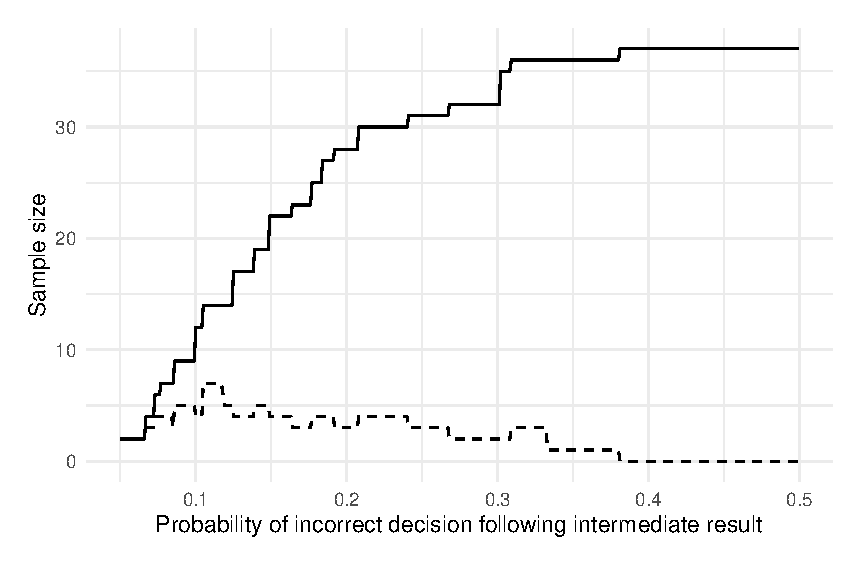
\includegraphics[scale=0.8]{./figures/eta_ns}
\caption{Minimum required sample size for a three-outcome design as a function of $\eta$ (solid line), along with the corresponding size of the intermediate zone $x_1 - x_0$ (dashed line).}
\label{fig:eta_ns}
\end{figure}

When $\eta = 0.5$, in which case we can only guess at the correct decision following a \emph{pause} outcome, the optimal sample size is $n = 52$. \footnote{We might have expected the three- and two-outcome designs to coincide at this point, and indeed this is the case if we employ a normal approximation for $\hat{\rho}$. When using exact binomial probabilities, as we have done here, the optimal three-outcome design has $x_0 = 31, x_1 = 32$, in comparison to the $x = 32$ of the two-outcome design. This suggests the true optimal $x$ for a two-outcome design lies in the interval $(31, 32)$} Figure \ref{fig:eta_ns} shows that a low value of $\eta$ is required to achieve a meaningful reduction in sample size. For example, for a 20\% reduction from the $n = 52$ two-outcome design down to $n = 41$, we would require $\eta = 0.2$. That is, we must be confident that following a \emph{pause} outcome, but with a true $\rho = \rho_i (i = 0,1)$, we will make the correct progression decision with a probability of 0.8. In the context of our simple one-parameter example, the estimate $\hat{\rho}$ is a sufficient statistic for $\rho$ and so we cannot obtain any other information relevant to this particular judgement. This would lead to $\eta = 0.5$, in which case the optimal three-outcome design will reduce to a two-outcome design.

We may expect $\eta < 0.5$ if measures of another variable in the trial, correlated with the variable of interest, are going to inform the progression decision following an \emph{pause} outcome. For example, patient adherence and retention may be correlated. If an \emph{pause} outcome was observed when assessing adherence but retention was seen to be high, we might infer the true adherence rate to be larger than the estimate. The extent of this will depend, however, on the strength of the correlation, which may be hard to judge at the design stage. 

To explore the implications of incorrectly assuming $\eta < 0.5$, we took each of the optimal designs found over the range $0 \leq \eta \leq 0.5$ and calculated their type I and II error rates under a true value of $\eta = 0.5$. These error rates are plotted in Figure \ref{fig:eta_true_ocs}. We find that error rates will be substantially inflated whenever $\eta$ was incorrectly assumed to be small enough to lead to a meaningful reduction in sample size. For example, if we incorrectly assume $\eta = 0.2$ when in fact $\eta = 0.5$ the `optimal' design will lead to actual type I and II error rates of 0.094 and 0.188, rather than the nominal 0.05 and 0.1.

\begin{figure}
\centering
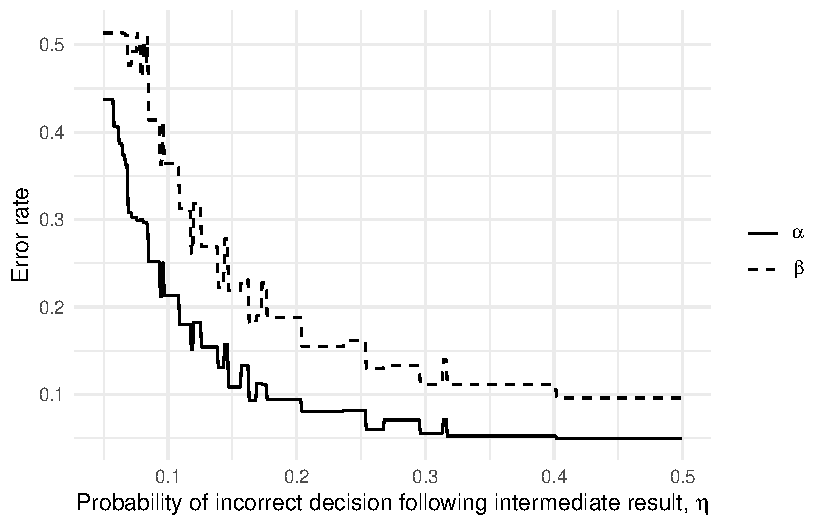
\includegraphics[scale=0.8]{./figures/eta_true_ocs}
\caption{Type I (solid line) and II (dashed line) error rates of optimal three-outcome designs for a range of assumed $\eta$, when in fact $\eta = 0.5$.}
\label{fig:eta_true_ocs}
\end{figure}

Given the challenges of estimating $\eta$ and the implications of doing it badly, we follow previous suggestions \cite{Sargent2001a, Dehbi2020} that a default assumption of $\eta = 0.5$ is appropriate and conclude that three-outcome progression criteria are not suitable for improving statistical efficiency in pilot trials.

\subsection{Incorporating other information}\label{sec:information}

We have argued that, without strong assumptions, using other sources of information to make progression decisions via an intermediate result will not improve statistical efficiency. We may, nevertheless, want to use such a procedure to allow this other information to inform the progression decision, rather then being ignored completely. For example, in addition to requiring sufficient adherence we may also want to see good recruitment and retention in the pilot trial. In the event of a \emph{pause} outcome when assessing adherence, we could then decide to proceed to the main trial only if the estimated recruitment and retention rates are large enough. A \emph{pause} outcome could also provide an opportunity for discussion amongst the various stakeholders (such as the trial team, steering committee and funder) to arrive at a collective decision on progression.

To facilitate this we can encourage the design to have an appropriate intermediate zone $| x_1 - x_0|$ by constraining the operating characteristic $\gamma = \gamma_L + \gamma_U$ defined in Table \ref{tab:ocs}, thus limiting the chance of making a conclusive \emph{stop} or \emph{go} decision when $\rho = \rho'$. With $\rho_0 = 0.5, \rho_1 = 0.7, \alpha \leq 0.05$ and $\beta \leq 0.1$ as before, we set $\rho' = (\rho_1 - \rho_0)/2 = 0.6$ and found optimal designs for a range of $\gamma^*$ while assuming throughout that $\eta = 0.5$. The sample sizes of these designs are plotted in Figure \ref{fig:gamma_ns}.

\begin{figure}
\centering
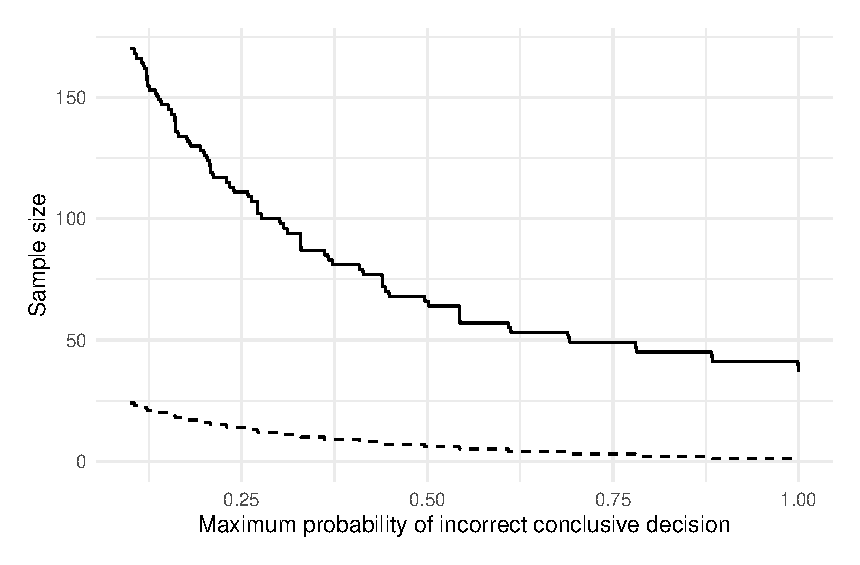
\includegraphics[scale=0.8]{./figures/gamma_ns}
\caption{Minimum required sample size for a three-outcome design as a function of $\gamma^*$ (solid line), along with the corresponding size of the intermediate zone $x_1 - x_0$ (dashed line).}
\label{fig:gamma_ns}
\end{figure}

When we set $\gamma^* = 1$, no intermediate zone is required and so the optimal design is the usual two-outcome design. As we decrease the nominal level on this constraint we permit an ever smaller probability of obtaining a conclusive \emph{stop} or \emph{go} outcome when $\rho = \rho'$. This leads to an increasing width of intermediate zone $|x_1 - x_0|$, alongside an increasing sample size. The required increase in sample size beyond the two-outcome design can be substantial. For example, to ensure a maximum 40\% chance of obtaining a conclusive result when $\rho = \rho'$, we must increase the sample size from $n = 52$ to $n = 98$. Providing such increases in sample size are considered worthwhile, we conclude that three-outcome designs can be used in pilot trials to allow other information and stakeholders to feed into progression decisions.

\subsection{Allowing for adjustments}

A final rationale for an intermediate outcome in pilot trials is to enable some modifications to be made prior to commencing the main trial. These could be adjustments to the trial design (e.g. to improve recruitment) or to the intervention itself (e.g. to improve adherence). The intermediate \emph{pause} outcome now leads to the decision to either \emph{stop} or to make these modifications and then \emph{go} to the main trial. Recall from Section \ref{sec:adjustments} that the effect of such an adjustment is denoted by $\tau$.

\subsubsection{Known adjustment effect}

Assume that the effect of adjustment $\tau$ is known \emph{a priori} and that $\eta = 0.5$. Considering the same problem as before ($\rho_0 = 0.5, \rho_1 = 0.7, \alpha^* = 0.05, \beta^* = 0.1, eta = 0.5$) we found optimal designs for a range of known adjustment effects spanning $\tau \in [0, 0.125]$. The required sample size of these designs is illustrated in Figure \ref{fig:tau_ns}. 

\begin{figure}
\centering
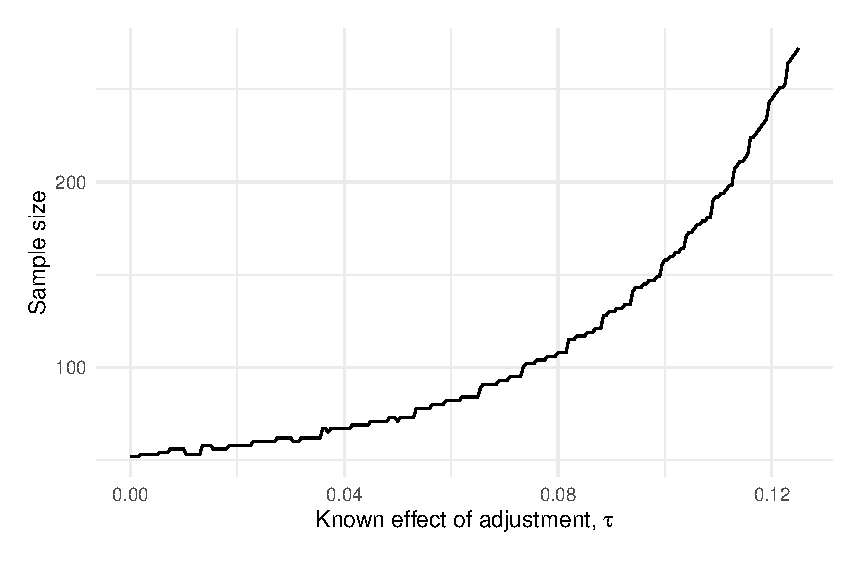
\includegraphics[scale=0.8]{./figures/tau_ns}
\caption{Minimum required sample size for a three outcome design as a function of the known adjustment effect $\tau$.}
\label{fig:tau_ns}
\end{figure}

When adjustments have no effect ($\tau = 0$), the optimal three-outcome design reduces to the usual \emph{stop/go} two-outcome design with $n = 52$. As $\tau$ increases the required sample size increases with it exponentially. We can see why this is when we look back at our error rate definitions in Equations \ref{eqn:alpha} and \ref{eqn:beta}, which show that $\alpha$ constrains the term $\PR(x_1 < \hat{\rho} ~|~ rho = \rho_0)$ while $\beta$ constrains the term $\PR(\hat{\rho} < x_0 ~|~ \rho = \rho_1 - \tau_{max})$. Note that this also implies we must have $\tau < \rho_1 - \rho_0$ in order to have both $\alpha < 0.5$ and $\beta < 0.5$.

\subsubsection{Partially known adjustment effect}

We now consider the case where the adjustment effect $\tau$ is known only up to an interval $\tau \in [\tau_{min}, \tau_{max}]$. We considered a range of values for $\tau_{min}$ from 0 up to 0.1 alongside a range of interval widths $\tau_{max} - \tau_{min}$ from 0 to 0.05. The resulting sample sizes are plotted in Figure \ref{fig:tau_part_ns}.

\begin{figure}
\centering
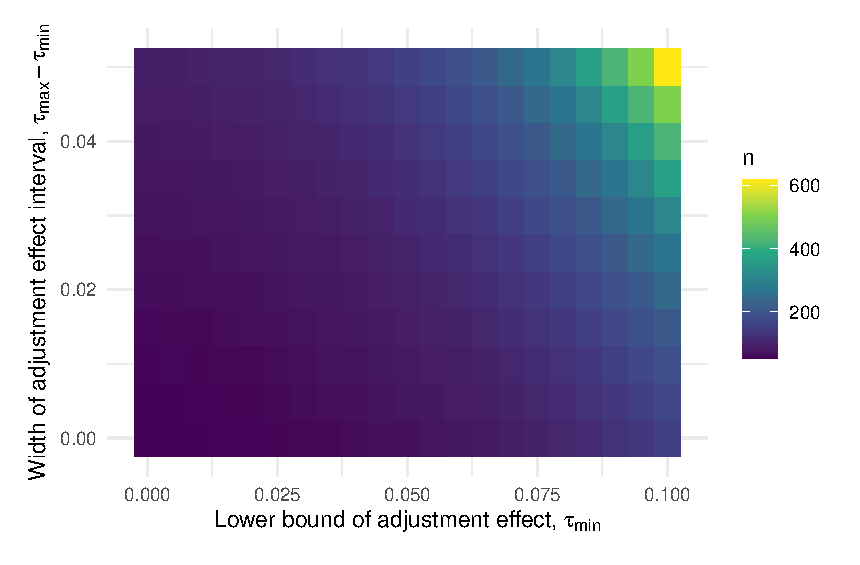
\includegraphics[scale=0.8]{./figures/tau_part_ns}
\caption{Minimum required sample size for a three outcome design as a function of the known adjustment effect $\tau$.}
\label{fig:tau_part_ns}
\end{figure}

We see that increasing the interval width leads to an increased sample size, and the rate at which this happens increases with the lower interval limit $\tau_{min}$. For example, moving from $[\tau_{min}, \tau_{max}] = [0, 0]$ to [0, 0.05] leads to a change in sample size from $n = 52$ to $n = 93$; which moving from   $[\tau_{min}, \tau_{max}] = [0.1, 0.1]$ to $[0.1, 0.15]$ takes us from $n = 158$ to $n = 620$. Figure \ref{fig:tau_part_ns} suggests that the main driver of sample size is the upper limit $\tau_{max}$, but changing $\tau_{min}$ while keeping this fixed can still lead to considerable changes in $n$. From example, $[\tau_{min}, \tau_{max}] = [0.05, 0.05]$ requires $n = 71$ while $[\tau_{min}, \tau_{max}] = [0.01, 0.05]$ requires $n = 87$.

\subsubsection{The case $\eta < 0.5$}

In the preceding subsections we have assumed that $\eta = 0.5$ following the arguments made in Section \ref{sec:efficiency}. In the context of allowing adjustments, however, we might argue that $\eta < 0.5$ is plausible since although we may not be able to learn anything about $\rho$ beyond what is provided by $\hat{\rho}$, we might learn something about the adjustment effect $\tau$ during the pilot. If we can assume this will reduce $\eta$, this will reduce the required sample size in a manner similar to the no-adjustment case discussed in Section \ref{sec:efficiency} (see supplementary material for more details). We must bear in mind, though, that learning about $\tau$ can only take us so far. Even in the extreme case where we can learn $\tau$ exactly, the residual uncertainty about $\rho$ will place a lower limit on our ability to make the correct decision following a \emph{pause} outcome.

We conclude that for three-outcome progression criteria to be useful in this context, the effect of the anticipated adjustment must be known (or at least estimated with little error) at the design stage if we are to avoid considerable inflation of error rates.\todo{Michelle - I have tried to moderate the conclusion here but if you're not happy we should discuss.}

\section{Discussion}\label{sec:discussion}

Assuming the adjustment effect $\tau$ is known \emph{a priori} will not always be tenable. On the contrary, a primary goal of many pilot trials is to identify \emph{unforeseen} problems and solutions to these. In this context, pre-specifying an upper threshold $x_1$ may make sense as this can help identify cases which are feasible enough, without modification, to proceed to the main trial. In contrast, the lower threshold $x_0$ appears somewhat arbitrary and may force inappropriate decisions. For example, if $x_0$ is set too high, we may be led to a \emph{stop} decision (i.e. $\hat{\rho} \leq x_0$) despite believing, based on what was seen in the pilot, that a certain modification would lead to an adjusted adherence rate greater than $\rho_1$.\todo{Michelle - for me, this is the key point on why pre-sepcified `adjust' rules shouldn't be recommended}
\footnote{See the supplementary material for some theoretical justification of this intuition.}


% Is it harder to choose hypotheses for feasibility parameters? And how should we dtermine OC constraints? Linking to power or subsequent sample size requirments may be one (partial) solution.

% Recognise that the testing framework is only a model. Sample size given should be taken as a minumum - might want more for other reasons, in which case thresholds should be adjusted. And in practice, adjustements might be made throughout the trial to try and work out what works. TCan our formal approach allow for this? Like a platform trial, adding in new arms (adjustments) as they become available and trying to find which works best.

% Could argue that three outcome designs always be used as they better reflect practice. But same argument will apply - the three outcome result should not be followed blindly, but interpreted as one piece of evidence.

We have shown how the three-outcome progression criteria commonly used in pilot trials can be viewed as three-outcome hypothesis tests, and described how related clinical trial designs from the phase II setting can be used (with some reformulation) to optimise these criteria and the pilot sample size. This allowed for a formal comparison to be made between three- and two-outcome designs for pilot trials. We have shown that three-outcome designs do not improve efficiency in comparison to the two-outcome alternative, but that three-outcome designs can be used to allow for a more realistic decision making process involving multiple sources of information and multiple stakeholders in the event of a borderline result if the cost of a larger sample size in comparison with the two-outcome alternative is deemed worthwhile. We have also shown that considerably larger sample sizes sample sizes are needed to facilitate making adjustments to the intervention or trial design following the pilot, particularly when the effect of such an adjustment is not known precisely in advance. \todo{Moderated conclusions to be clearer that three-outcomes have some clear benefits which are offset by increased sample size required.}

In order to apply the proposed method in practice, we need to specify null and alternative hypotheses and put constraints on the type I and II error rates. Specifying hypotheses for feasibility parameters like adherence rates might be challenging. Generally, there will be no default choice for the null (as opposed to when considering efficacy, when the null hypothesis is typically no difference to standard care), and the concept of Minimal Clinically Important Difference, which often guides the choice of target difference in efficacy, will not be applicable for feasibility. It may help to begin by determining the midpoint $\rho_m = (\rho_0 + \rho_1)/2$ which we would consider a borderline value and where we would ideally like to observe a \emph{pause} decision, determine the width of the interval $|\rho_1 - \rho_0|$, and then choose type I and II error constraints based on the relative impact of these errors when defined with respect to $\rho_0$ and $\rho_1$. Having determined these values, one can find optimal designs for a range of constraints on the third operating characteristic $\gamma$ (the probability of observing a   \emph{pause} decision when $\rho = \rho_m$) as shown in Figure\ref{fig:gamma_ns}.

As an alternative means to improve efficiency in pilot trials, adaptive designs incorporating one or more interim analysis may be useful. These would allow the pilot trial to finish early if interim data gave a sufficiently strong indication of feasibility (or lack thereof). The terminal progression criteria in such an adaptive design could be made three-outcome to allow other information to be incorporated at that stage, and indeed this aligns with Sargent et al.'s \cite{Sargent2001} proposal which included both one and two stage versions of their design. 

To determine if and how the intervention or trial design should be adjusted before the main trial, one could consider a multi-arm pilot trial where each arm implements a different proposed adjustment. This would then inform which adjustment, if any, should be implemented for the main trial. A multi-arm trial will require a larger sample size than a standard two-arm pilot, but this may be mitigated against somewhat by incorporating interim analyses in a Multi-Arm Multi-Stage (MAMS) design. Alternatively, a factorial pilot trial could be used to identify the optimal selection of adjustments to take forward. These solutions would help address the problem of not knowing the effect of some proposed adjustments, but would still require their nature to be known in advance. When a new and unanticipated adjustment is proposed following the pilot trial, undertaking a second pilot to establish that it works as expected may be the best course of action. A similar strategy has been suggested in the context of phase II drug trials \cite{Brown2012}.

An alternative approach to meeting these objectives is to design and analyse the pilot trial under a Bayesian framework\cite{Hampson2017, Wilson2021}. This could improve efficiency by allowing external information or expert knowledge to be incorporated into decision making, and would enable a flexible approach to analysis that does not require adherence to pre-specified decision rules. Willan and Thabane \cite{Willan2020} do not consider the question of optimising pilot sample size, but show through an example how a Bayesian analysis of pilot data can help quantify uncertainty around feasibility parameters and use their posterior distributions to design the main trial. 

%One conclusion of this work is that standard two-outcome hypothesis tests should be used to determine progression criteria and the pilot trial sample size. The standard approach to this requires a null and alternative hypothesis to be specified, alongside constraints on type I and II error rates which refelct the consequences of these errors. An alternative approach is to instead determine the parameter value at which we would be indifferent between making \emph{stop} and \emph{go} and set the progression criteria threshold to that same value, leading to a test with 50\% power at that point. The sample size can then be chosen to give a desired probability of progression at some other point in the parameter space such as the point null hypothesis \cite{Willan1994}. It seems plausible that this is how progression criteria are currently determined in practice.

Our work has been motivated by external pilot trials assessing the feasibility but may be equally relevant to other settings, such as phase II drug trials, where the parameter of interest is some measure of efficacy. Making post trial adjustments to improve efficacy could then take the form of, for example, changing eligibility criteria in an attempt to focus on a subgroup of patients who stand to benefit most from the treatment. Although our findings should also extend apply equally to internal  pilot trials, the error rates of the final analysis of effectiveness may be affected by a formal internal pilot analysis of a correlated endpoint like adherence. Finally, we expect our conclusions to carry over from the univariate setting considered here to the more general multivariate setting, where several progression criteria are applied simultaneously, although it has been shown that such multivariate tests may be counter-intuitively inefficient \cite{Wilson2021a}.

%%%%%%%%%%%%%%%%%%%%%%%%%%%%%%%%%%%%%%%%%%%%%%
%%                                          %%
%% Backmatter begins here                   %%
%%                                          %%
%%%%%%%%%%%%%%%%%%%%%%%%%%%%%%%%%%%%%%%%%%%%%%

\begin{backmatter}

\section*{Competing interests}
  The authors declare that they have no competing interests.

\section*{Author's contributions}
    Text for this section \ldots

\section*{Acknowledgements}
  Text for this section \ldots
  
%%%%%%%%%%%%%%%%%%%%%%%%%%%%%%%%%%%%%%%%%%%%%%%%%%%%%%%%%%%%%
%%                  The Bibliography                       %%
%%                                                         %%
%%  Bmc_mathpys.bst  will be used to                       %%
%%  create a .BBL file for submission.                     %%
%%  After submission of the .TEX file,                     %%
%%  you will be prompted to submit your .BBL file.         %%
%%                                                         %%
%%                                                         %%
%%  Note that the displayed Bibliography will not          %%
%%  necessarily be rendered by Latex exactly as specified  %%
%%  in the online Instructions for Authors.                %%
%%                                                         %%
%%%%%%%%%%%%%%%%%%%%%%%%%%%%%%%%%%%%%%%%%%%%%%%%%%%%%%%%%%%%%

% if your bibliography is in bibtex format, use those commands:
\bibliographystyle{bmc-mathphys} % Style BST file (bmc-mathphys, vancouver, spbasic).
\bibliography{DTWrefs}      % Bibliography file (usually '*.bib' )
% for author-year bibliography (bmc-mathphys or spbasic)
% a) write to bib file (bmc-mathphys only)
% @settings{label, options="nameyear"}
% b) uncomment next line
%\nocite{label}

% or include bibliography directly:
% \begin{thebibliography}
% \bibitem{b1}
% \end{thebibliography}

%%%%%%%%%%%%%%%%%%%%%%%%%%%%%%%%%%%
%%                               %%
%% Figures                       %%
%%                               %%
%% NB: this is for captions and  %%
%% Titles. All graphics must be  %%
%% submitted separately and NOT  %%
%% included in the Tex document  %%
%%                               %%
%%%%%%%%%%%%%%%%%%%%%%%%%%%%%%%%%%%

%%
%% Do not use \listoffigures as most will included as separate files

\section*{Figures}
  \begin{figure}[h!]
  \caption{\csentence{Sample figure title.}
      A short description of the figure content
      should go here.}
      \end{figure}

\begin{figure}[h!]
  \caption{\csentence{Sample figure title.}
      Figure legend text.}
      \end{figure}

%%%%%%%%%%%%%%%%%%%%%%%%%%%%%%%%%%%
%%                               %%
%% Tables                        %%
%%                               %%
%%%%%%%%%%%%%%%%%%%%%%%%%%%%%%%%%%%

%% Use of \listoftables is discouraged.
%%
\section*{Tables}
\begin{table}[h!]
\caption{Sample table title. This is where the description of the table should go.}
      \begin{tabular}{cccc}
        \hline
           & B1  &B2   & B3\\ \hline
        A1 & 0.1 & 0.2 & 0.3\\
        A2 & ... & ..  & .\\
        A3 & ..  & .   & .\\ \hline
      \end{tabular}
\end{table}

%%%%%%%%%%%%%%%%%%%%%%%%%%%%%%%%%%%
%%                               %%
%% Additional Files              %%
%%                               %%
%%%%%%%%%%%%%%%%%%%%%%%%%%%%%%%%%%%

%\section*{Additional Files}
%  \subsection*{Additional file 1 --- Sample additional file title}
%%    Additional file descriptions text (including details of how to
%    view the file, if it is in a non-standard format or the file extension).  This might
%    refer to a multi-page table or a figure.
%
%  \subsection*{Additional file 2 --- Sample additional file title}
%    Additional file descriptions text.


\end{backmatter}
\end{document}